\section{Evaluation}
\label{sec:eval}

\begin{figure*}[!t]
  \centering
  \begin{subfigure}[t]{0.48\linewidth}
    \centering
    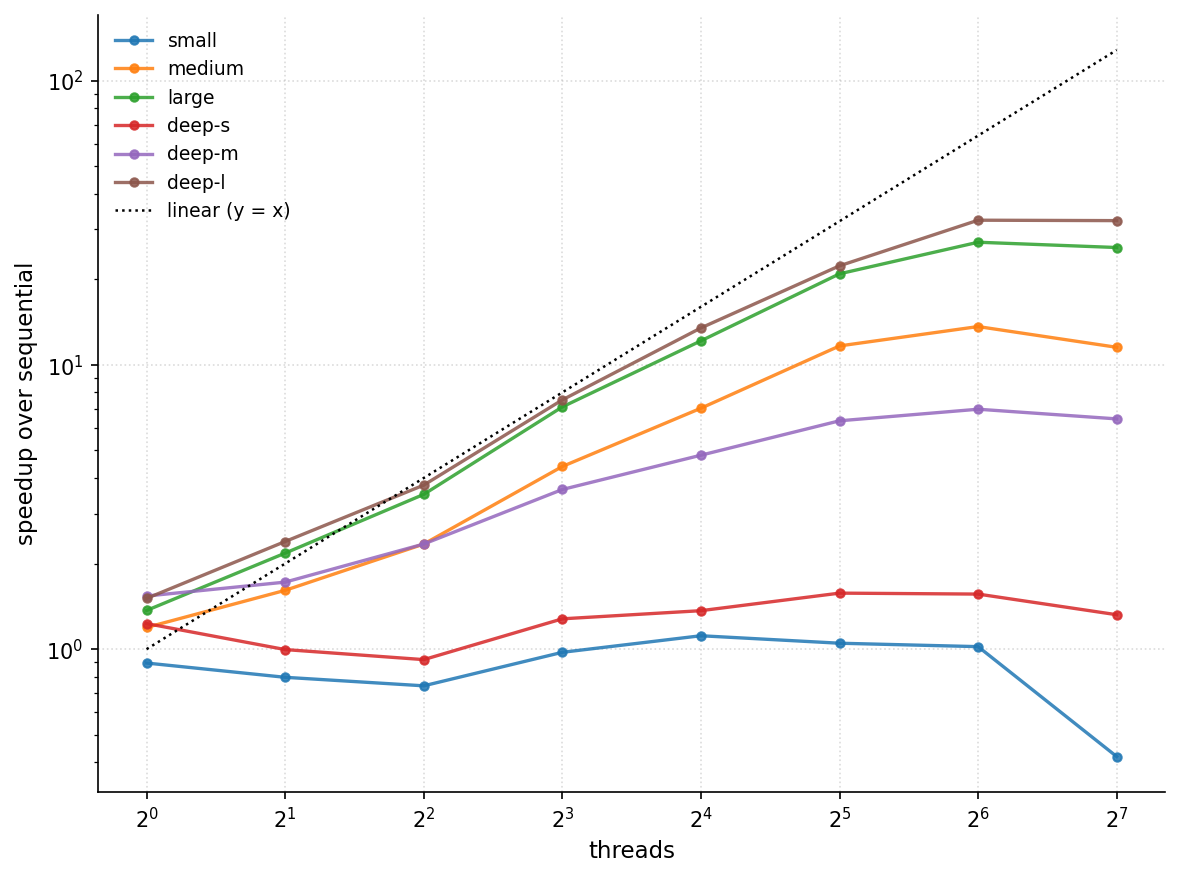
\includegraphics[width=\linewidth]{plots/random_loglog.png}
    \caption{Runtime vs. thread count (log-log).}
    \label{fig:random:loglog}
  \end{subfigure}\hfill
  \begin{subfigure}[t]{0.48\linewidth}
    \centering
    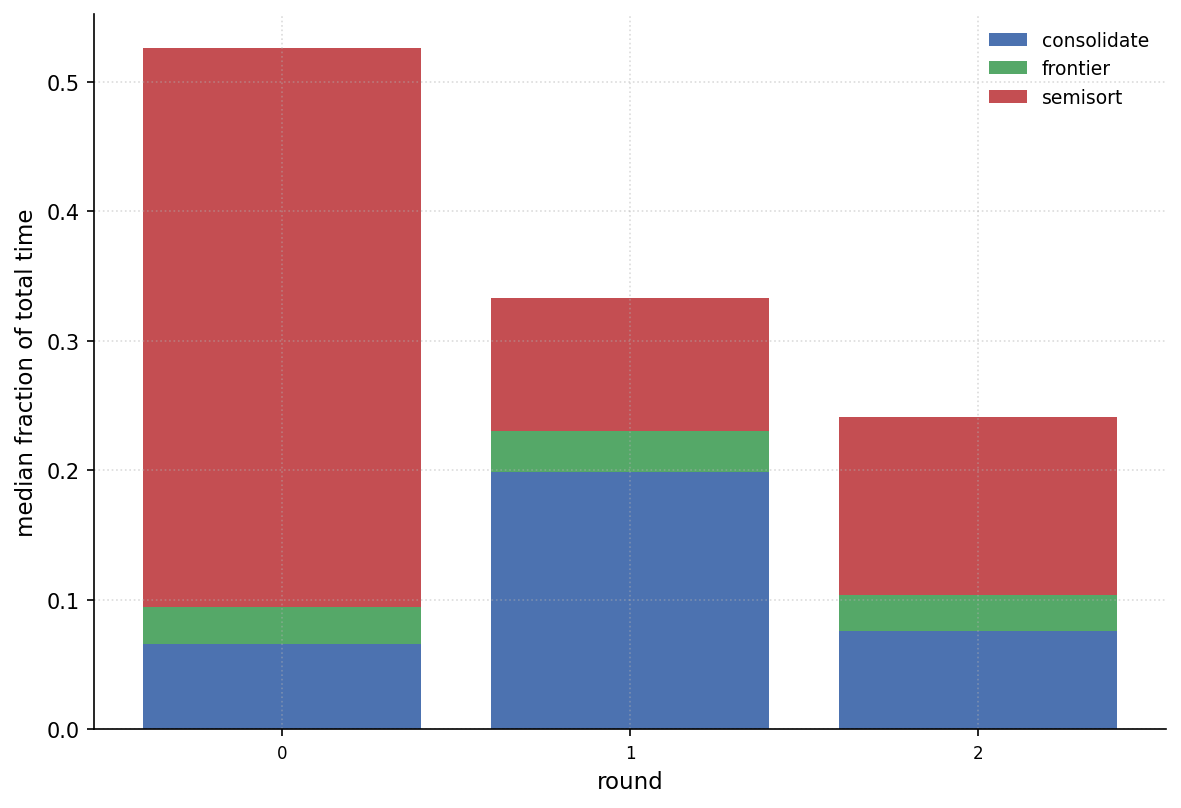
\includegraphics[width=\linewidth]{plots/random_phasebar_combined.png}
    \caption{Per-phase time breakdown.}
    \label{fig:random:phasebar}
  \end{subfigure}
  \caption{Random leaf-only benchmarks on binary nodes.}
  \label{fig:random}
\end{figure*}

In this section, we evaluate our parallel congruence closure algorithm on a
number of benchmarks in order to answer the following research questions:

\begin{itemize}
  \item \textbf{RQ1:} Does our parallel congruence closure algorithm achieve a
  meaningful speedup over a sequential implementation and how does this speedup
  scale with the number of threads?
  \item \textbf{RQ2:} What characterizes the type of benchmark that our parallel
  congruence algorithm performs well on?
  \item \textbf{RQ3:} How does our parallel congruence closure algorithm perform
  on real-world benchmarks, such as those from an SMT solver or an equality
  saturation engine?
\end{itemize}

We demonstrate the efficacy and limitations of our approach through a wide
selection of benchmarks on various workloads. In \autoref{sec:eval:random}, we
discuss a randomly generated benchmark suite to stress test our algorithm. In
\autoref{sec:eval:synthetic}, we discuss a synthetic benchmark suite that allows
us to dial up the depth and width of the benchmark to better understand how
these parameters affect the performance of our algorithm. Finally, in
\autoref{sec:eval:egg}, we discuss a set of benchmarks from the Herbie floating
point optimizer~\cite{herbie} that in turn calls the egg equality saturation
engine~\cite{egg}.

All experiments were performed on the Bridges-2 supercomputer on nodes with 128
cores and 256 GB RAM~\cite{bridges}. The node consisted of NVMe SSD (3.84TB);
Mellanox ConnectX-6 HDR Infiniband 200Gb/s Adapter; and two AMD EPYC 7742 CPUS (
each with 64 cores, 2.25-3.40GHz, 256MB L3, and 8 memory channels).

For each run, we perform 1 warmup run and 5 timed runs, and we report the median of the 5 timed runs.

\subsection{Leaf-only Equalities on Binary Nodes}~\label{sec:eval:random}

Our first set of benchmarks is parameterized by several parameters. $l$ denotes
the number of leaves---i.e. the ``variables'' that appear within terms. $w$
denotes the \emph{width} of the benchmark: how many equalities are initially
given before computing their congruence closure. The parameter $n$ denotes the
total number of \emph{nodes}, which are non-leaf terms (e.g. function
applications). The \emph{depth} $d$ denotes the depth of the terms, or how many
nested function applications appear in the term. For example, the term $f(g(x))$
has depth 2, and the term $x$ (a single variable) has depth 0. The parameter $f$
denotes the number of function symbols. Finally, the parameter $p$ denotes the
number of software threads.

We now describe the experiments. We fix $f = 16$ and the arity of each function
symbol to 2. For one set of experiments, we stratify our workloads into
different size classes, which are shown in Table~\ref{tab:workloads}.

\begin{table}[t]
  \centering
  \begin{tabular}{l r r r r r}
    \toprule
    workload & $n_{\text{leaves}}$ & $n_{\text{nodes}}$ & $n_{\text{merges}}$ &
    depth & $n_{\text{fns}}$ \\
    \midrule
    \texttt{small}   &      1\,000 &     10\,000 &      2\,000 & 1 &  4 \\
    \texttt{deep-s}  &      1\,000 &     10\,000 &      2\,000 & 3 &  4 \\
    \texttt{medium}  &     10\,000 &    200\,000 &     20\,000 & 1 &  8 \\
    \texttt{deep-m}  &     10\,000 &    200\,000 &     20\,000 & 3 &  8 \\
    \texttt{large}   &     50\,000 &  1\,000\,000 &    100\,000 & 3 & 16 \\
    \texttt{deep-l}  &     50\,000 &  1\,000\,000 &    100\,000 & 3 & 16 \\
    \texttt{xl-d3}   &    100\,000 &  2\,000\,000 &    200\,000 & 3 & 16 \\
    \texttt{2xl-d3}  &    200\,000 &  4\,000\,000 &    400\,000 & 3 & 16 \\
    \texttt{4xl-d3}  &    400\,000 &  8\,000\,000 &    800\,000 & 3 & 16 \\
    \texttt{8xl-d3}  &    800\,000 & 16\,000\,000 & 1\,600\,000 & 3 & 16 \\
    \texttt{16xl-d3} &  1\,600\,000 & 32\,000\,000 & 3\,200\,000 & 3 & 16 \\
    \bottomrule
  \end{tabular}
  \caption{Synthetic workload parameters. Each workload is a layered random
  binary-tree DAG with $n_{\text{leaves}}$ \texttt{x}-leaves plus
  $n_{\text{leaves}}$ \texttt{y}-leaves at the base, $n_{\text{nodes}}$ function
  nodes distributed across \emph{depth} levels with $n_{\text{fns}}$
  uniformly-chosen operators per level, and $n_{\text{merges}}$ random
  initial-union pairs (half \texttt{x}-\texttt{x}, half \texttt{y}-\texttt{y}).
  All workloads use a fixed merge-density ratio $n_{\text{merges}} /
  n_{\text{leaves}} = 2$ and a constant scaling $n_{\text{nodes}} /
  n_{\text{leaves}} = 20$.}
  \label{tab:workloads}
\end{table}

\as{double check that the numbers in this table are correct}
% Architecture:                x86_64
%   CPU op-mode(s):            32-bit, 64-bit
%   Address sizes:             52 bits physical, 57 bits virtual
%   Byte Order:                Little Endian
% CPU(s):                      192
%   On-line CPU(s) list:       0-191
% Vendor ID:                   GenuineIntel
%   Model name:                Intel(R) Xeon(R) 6975P-C
%     CPU family:              6
%     Model:                   173
%     Thread(s) per core:      2
%     Core(s) per socket:      96
%     Socket(s):               1
%     Stepping:                1
%     CPU(s) scaling MHz:      24%
%     CPU max MHz:             3900.0000
%     CPU min MHz:             800.0000
%     BogoMIPS:                5400.00
%     Flags:                   fpu vme de pse tsc msr pae mce cx8 apic sep mtrr pge mca cmov pat pse36 clflush dts acpi mmx fxsr sse sse2 ss ht tm pbe syscall nx pdpe1gb rdtscp lm constant_tsc 
%                              art arch_perfmon pebs bts rep_good nopl xtopology nonstop_tsc cpuid aperfmperf tsc_known_freq pni pclmulqdq dtes64 monitor ds_cpl vmx smx est tm2 ssse3 sdbg fma c
%                              x16 xtpr pdcm pcid dca sse4_1 sse4_2 x2apic movbe popcnt tsc_deadline_timer aes xsave avx f16c rdrand lahf_lm abm 3dnowprefetch cpuid_fault epb cat_l3 cat_l2 cdp_
%                              l3 intel_ppin cdp_l2 ssbd mba ibrs ibpb stibp ibrs_enhanced tpr_shadow flexpriority ept vpid ept_ad fsgsbase tsc_adjust bmi1 avx2 smep bmi2 erms invpcid cqm rdt_a
%                               avx512f avx512dq rdseed adx smap avx512ifma clflushopt clwb intel_pt avx512cd sha_ni avx512bw avx512vl xsaveopt xsavec xgetbv1 xsaves cqm_llc cqm_occup_llc cqm_m
%                              bm_total cqm_mbm_local split_lock_detect user_shstk avx_vnni avx512_bf16 wbnoinvd dtherm ida arat pln pts hwp hwp_act_window hwp_epp hwp_pkg_req vnmi avx512vbmi u
%                              mip pku ospke waitpkg avx512_vbmi2 gfni vaes vpclmulqdq avx512_vnni avx512_bitalg tme avx512_vpopcntdq la57 rdpid bus_lock_detect cldemote movdiri movdir64b enqcm
%                              d fsrm md_clear serialize tsxldtrk pconfig arch_lbr ibt amx_bf16 avx512_fp16 amx_tile amx_int8 flush_l1d arch_capabilities
% Virtualization features:     
%   Virtualization:            VT-x
% Caches (sum of all):         
%   L1d:                       4.5 MiB (96 instances)
%   L1i:                       6 MiB (96 instances)
%   L2:                        192 MiB (96 instances)
%   L3:                        480 MiB (1 instance)
% NUMA:                        
%   NUMA node(s):              3
%   NUMA node0 CPU(s):         0-31,96-127
%   NUMA node1 CPU(s):         32-63,128-159
%   NUMA node2 CPU(s):         64-95,160-191
% Vulnerabilities:             
%   Gather data sampling:      Not affected
%   Ghostwrite:                Not affected
%   Indirect target selection: Not affected
%   Itlb multihit:             Not affected
%   L1tf:                      Not affected
%   Mds:                       Not affected
%   Meltdown:                  Not affected
%   Mmio stale data:           Not affected
%   Old microcode:             Vulnerable
%   Reg file data sampling:    Not affected
%   Retbleed:                  Not affected
%   Spec rstack overflow:      Not affected
%   Spec store bypass:         Mitigation; Speculative Store Bypass disabled via prctl
%   Spectre v1:                Mitigation; usercopy/swapgs barriers and __user pointer sanitization
%   Spectre v2:                Mitigation; Enhanced / Automatic IBRS; IBPB conditional; PBRSB-eIBRS Not affected; BHI BHI_DIS_S
%   Srbds:                     Not affected
%   Tsa:                       Not affected
%   Tsx async abort:           Not affected
%   Vmscape:                   Mitigation; IBPB before exit to userspace

Our first experiment plots the speedup over sequential baseline for each of these size classes with the number of processes fixed at $p = 192$. The results are shown in Figure~\ref{fig:width-speedup}: As we can see, the speedup over baseline scales rougly logarithmically with scale factor. As we see, there is a relative slowdown past scale factor 64x, at which point both programs become memory-bound. In particular, Granite Rapids Intel(R) Xeon(R) 6975P-C has a 480MB shared L3 cache, and the 16x scale factor workload maintains 32M nodes $\times$ 16 bytes per node $\approx$ 512MB, already exceeding the L3 cache. Thus past this point both variants (baseline and BSP) become memory-bound.

It is striking that parallel speedup increases monotonically with scale factor, well past the point where are hardware threads are saturated. This suggests that the per-round overheads are poorly amortized at small sizes. We validate this hypothesis in the following set of benchmarks, where

This is because the per-round overhead is quite high relative to other d



$l$, the numbers of ``leaves'' (i.e. the ) Our first set of benchmarks is a
synethetic benchmark that generates $w$ equalities of the form $i = j$ where
both $i$ is sampled uniformly at random from the range $f$.

\as{update \autoref{fig:random} when we have all the results for XL benchmarks.}


\autoref{fig:random:loglog} shows the runtime of our parallel congruence closure
We observe that on workloads with more nodes, our algorithm achieves a close to
linear speedup over the sequential version. This plateaus at around 64 threads,
for instance, 32-XL achieves a speedup of TODO\% on 64 threads and TODO\% on 128
threads.

While varying the number of nodes, leads to better speedups, the results for
varying the depth is more complicated. For instance, while \texttt{deep-s} and
\texttt{deep-l} achieve greater speedups than their less deep counterparts,
\texttt{deep-m} achieves a smaller speedup than \texttt{medium}. This is likely
because the depth of the benchmark affects the number of rounds of congruence
closure. Our algorithm only parallelizes over the merges within a round, but not
over the total number of rounds. We evaluate this further in
\autoref{sec:eval:synthetic}.

Finally, \autoref{fig:random:phasebar} shows the time breakdown in each round.
It takes the median percentage of time per round from all of the benchmarks.
We measure three rounds: (a) frontier is the parallel \texttt{filter} to gather
the frontier of changed classes, (b) semisort is the parallel semisort to group
parent e-nodes by their current, and (c) consolidate is the parallel pass to union
together all pairs of the same class in the semisort output. We notice that the
semisort is the most expensive phase, taking around TODO\% of the time, while
the frontier and consolidate phases take around TODO\% and TODO\% respectively.
This suggests that optimizing the semisort phase could lead to significant
performance improvements.

We notice that semisort is initially the largest phase in the first round, but
as we get into later rounds it becomes cheaper as we have fewer and fewer nodes
in the frontier.

\subsection{Varying Depth and Width}~\label{sec:eval:synthetic}

\begin{figure*}[!t]
  \centering
  \begin{subfigure}[t]{0.48\linewidth}
    \centering
    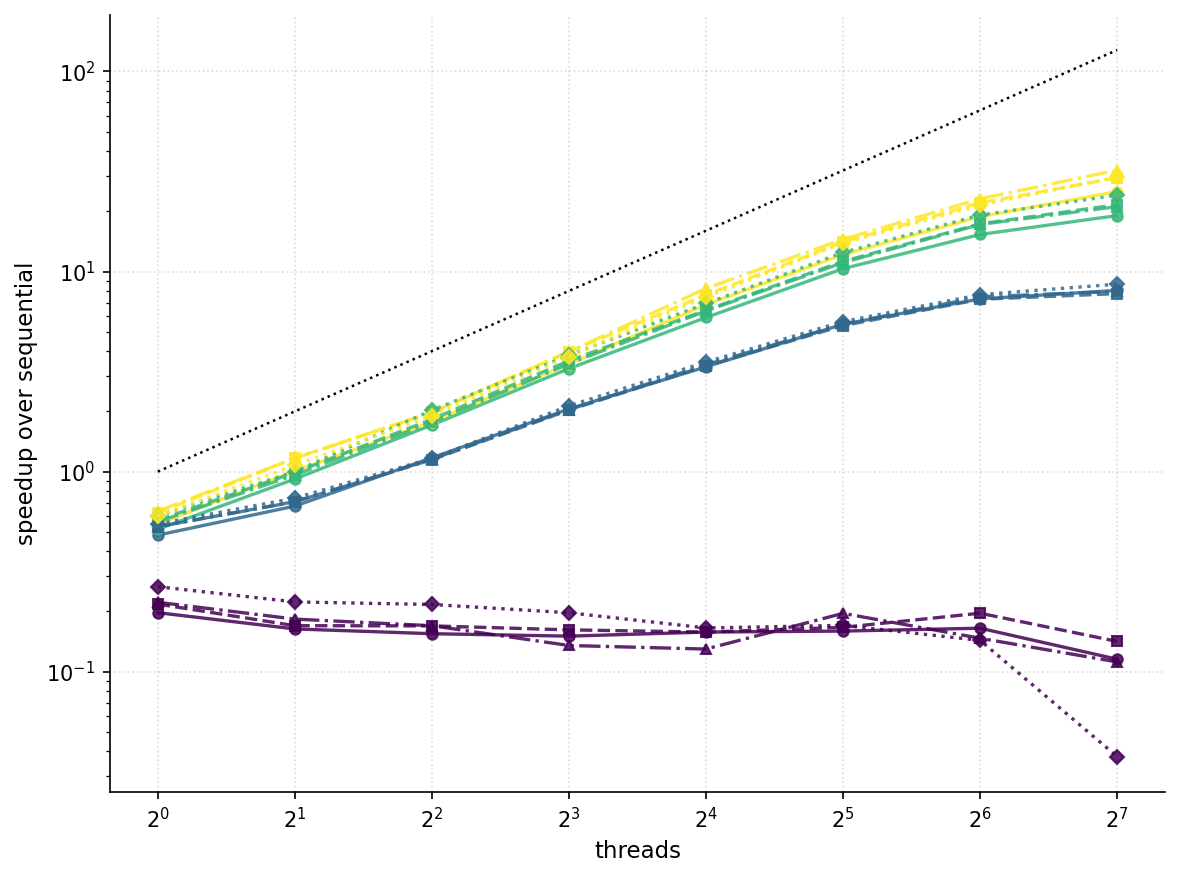
\includegraphics[width=\linewidth]{plots/cube_decomp_loglog.png}
    \caption{Runtime vs. thread count (log-log).}
    \label{fig:cube:loglog}
  \end{subfigure}\hfill
  \begin{subfigure}[t]{0.48\linewidth}
    \centering
    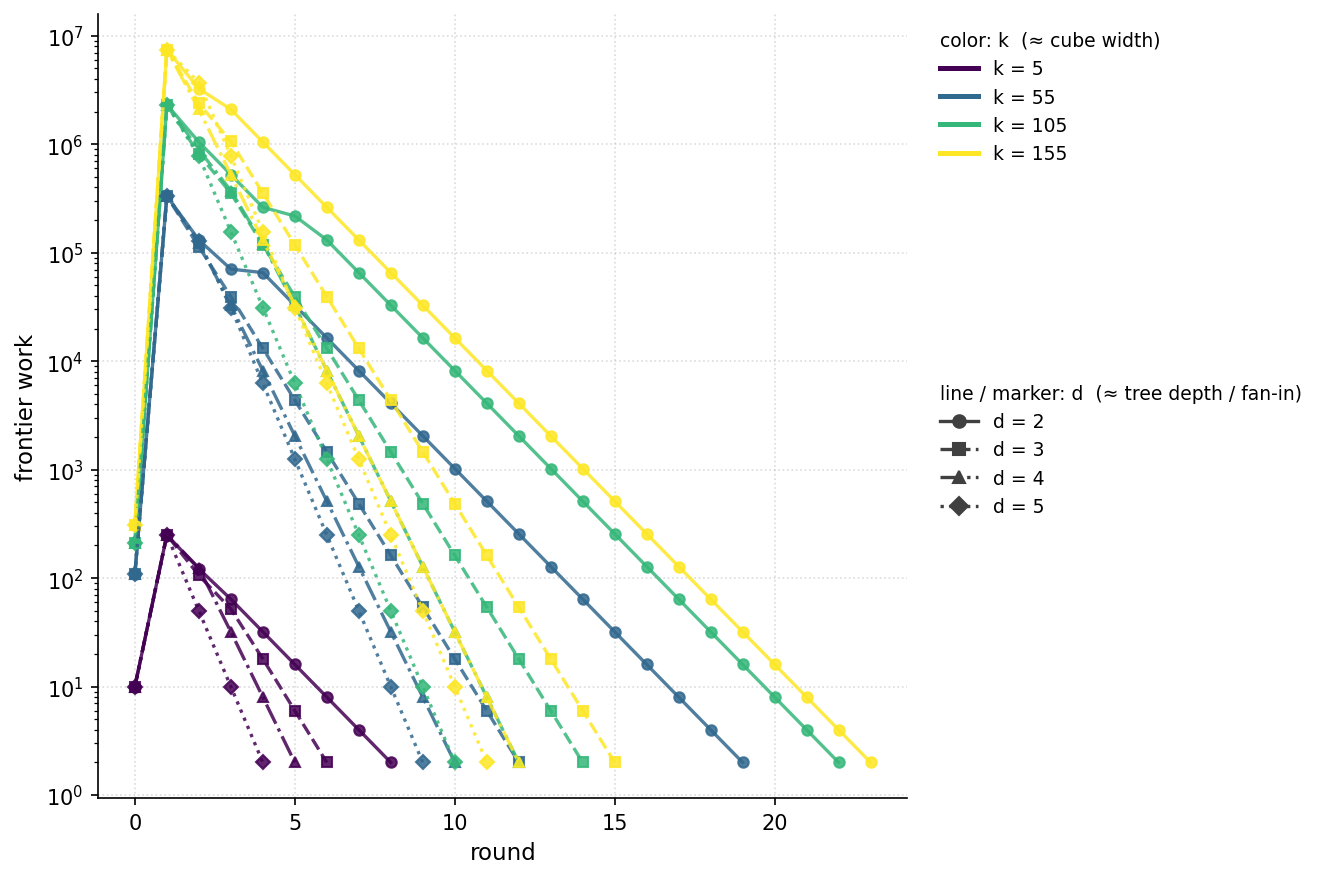
\includegraphics[width=\linewidth]{plots/cube_decomp_round_sizes.png}
    \caption{Per-round merge counts.}
    \label{fig:cube:rounds}
  \end{subfigure}
  \caption{Synthetic benchmarks varying depth and width.}
  \label{fig:cube}
\end{figure*}

To better understand the relationship between the depth (i.e. number of rounds of congruence closure)
and the width (i.e. number of merges per round) of the benchmark and the performance of our algorithm, we design a synthetic benchmark suite that allows us to dial up these parameters.

Our benchmark suite is based on the example in \autoref{ex:formula}. We create a benchmark with $2k$ leaves $a_1, \ldots, a_k$ and $b_1, \ldots, b_k$, and we assert the equalities $a_i = b_i$ for all $i$. We then have a single disequality between two terms built from $f$ and $g$. The disequality compares two applications of $g$, whose four arguments are the $f$-terms over the index set $\{1, ..., k\}^2$. The expected outcome is \texttt{unsat}. Then we create a $3^k$ terms of the form $f(a_i, a_j, a_k)$, which must be congruent to the corresponding $f(b_i, b_j, b_k)$ terms. Thus, $k$ parameterizes the width of the benchmark, as it controls how many merges are implied by the initial $k$ equalities. The depth is parameterized by some $d$ which controls how many nested $g$ applications we have. Each round will have $\frac1d$ of the merges of the previous round, so a larger
$d$ means a slower depth. We can observe this in \autoref{fig:cube:rounds}.

\autoref{fig:cube:loglog} shows the runtime of our parallel congruence closure algorithm on this benchmark suite. We observerve that increasing $k$ and hence the width of the benchmark leads to better speedups, while decreasing $d$ and hence increasing the depth of the benchmark has minimal impact. We achieve speedups of up to \_ on 128 cores for $k=155$ and $d=$TODO. This suggests that our algorithm performs well on benchmarks with a large number of merges per round, and is not significantly affected by the total number of rounds of congruence closure.


% We can then nest this structure to create more rounds of congruence closure. For instance, we can have a disequality between two applications of $g$ whose arguments are the $f(a_i, a_j, a_k)$ terms, which would require us to first merge all of the $f$-terms before we can merge the two $g$-terms. This would give us a benchmark with depth 2. We can then repeat this process to create benchmarks with depth 3, 4, and so on.

% Finally, we have a single disequality between two terms built from $f$ and $g$. The disequality compares two applications of $g$, whose four arguments are the $f$-terms over the index set $\{1, ..., k\}^3$. The expected outcome is \texttt{unsat}.


\subsection{Egg}~\label{sec:eval:egg}

\begin{figure*}[!t]
  \centering
  \begin{subfigure}[t]{0.48\linewidth}
    \centering
    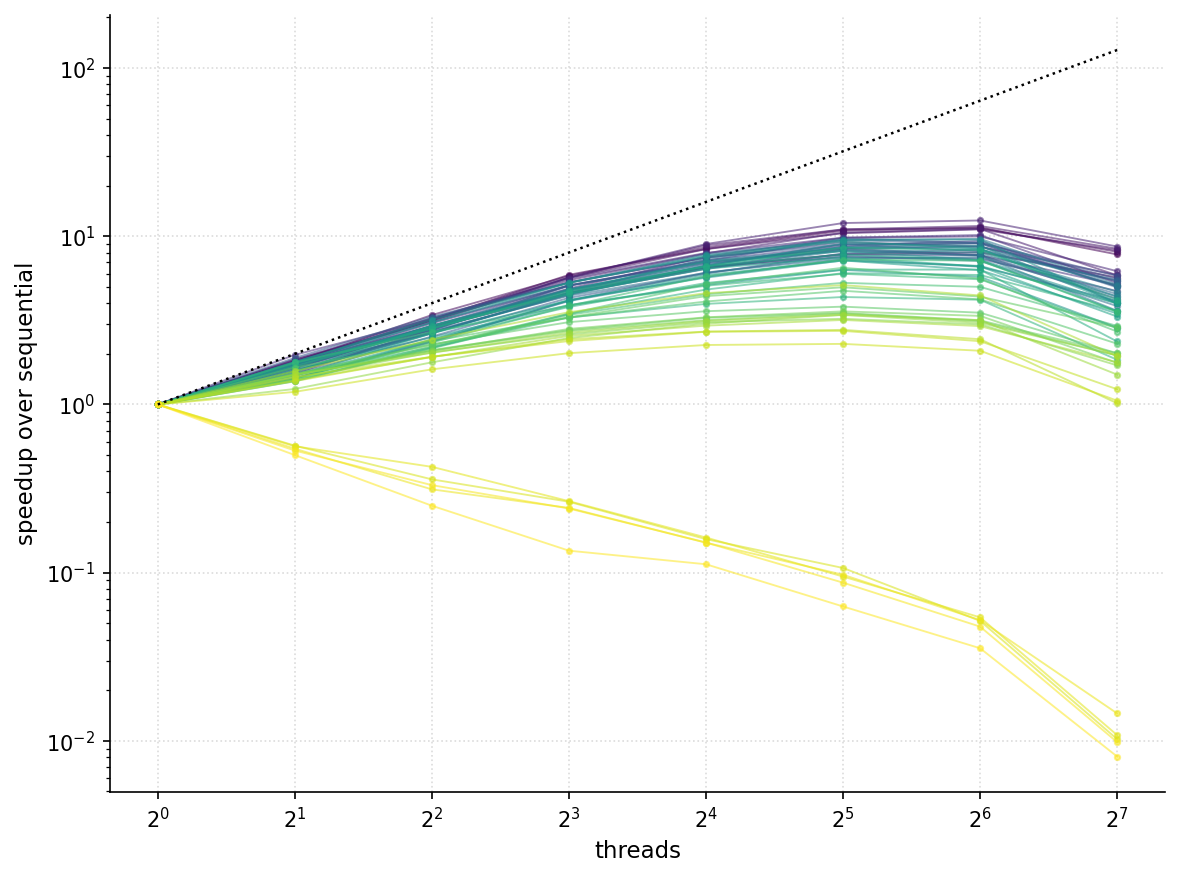
\includegraphics[width=\linewidth]{plots/egg_loglog.png}
    \caption{Runtime vs. thread count (log-log).}
    \label{fig:egg:loglog}
  \end{subfigure}\hfill
  \begin{subfigure}[t]{0.48\linewidth}
    \centering
    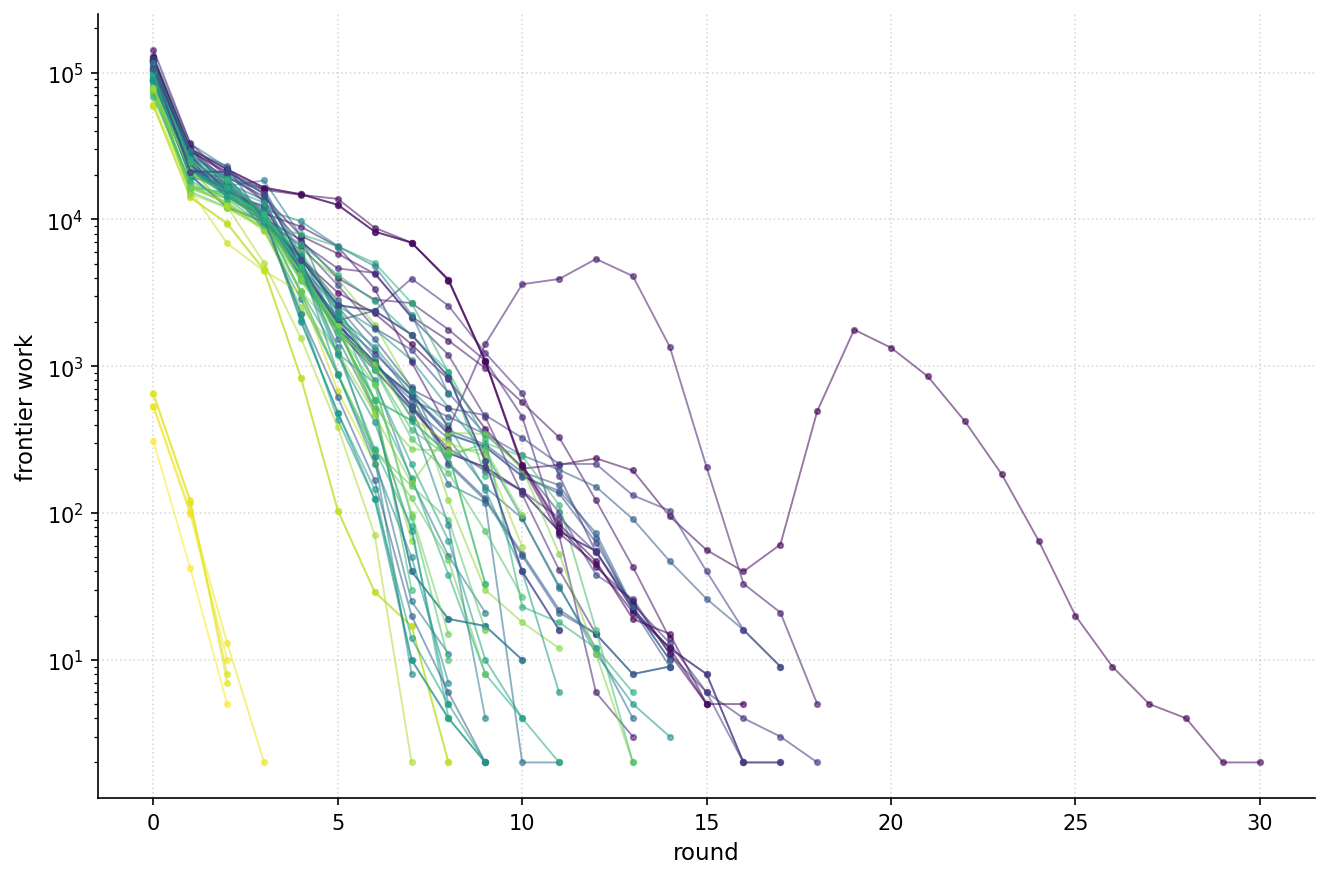
\includegraphics[width=\linewidth]{plots/egg_round_sizes.png}
    \caption{Per-round merge counts.}
    \label{fig:egg:rounds}
  \end{subfigure}
  \caption{Herbie/egg equality saturation benchmarks.}
  \label{fig:egg}
\end{figure*}